\subsection{Field}
Field er en abstrakt klasse, som alle felter i spillet nedarver fra. Klassen indeholder attributterne: title, beskrivelse, farve og id. Ownable som også er en abstrakt klasse nedarver fra Field, da det er en undergruppe af felter, der kan ejes af spillerene (se figur \ref{fig:fieldArv}).

\begin{figure}[!h]
    \centering
    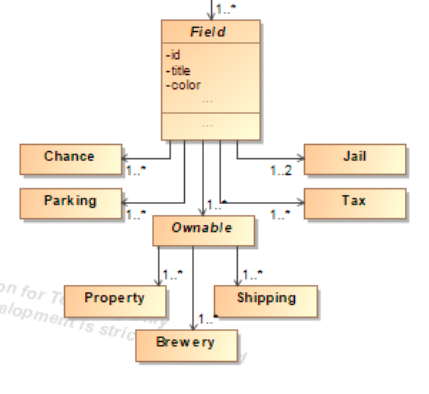
\includegraphics{sources/7_implementering/field-nedarvning.PNG}
    \caption{Klassediagram der viser nedarvningshiearkiet af Field}
    \label{fig:fieldArv}
\end{figure}

Felterne er delt op i 8 grupper.

Ikke muligt at eje:

\begin{itemize}
    \item Jail
    \item Parking
    \item Start
    \item Tax
    \item Chance
\end{itemize}

Muligt at eje:
\emph{Nedenstående felter vil blive gennemgået i afsnit 7.2}

\begin{itemize}
    \item Property
    \item Brewery
    \item Shipping
\end{itemize}



Felterne i sig selv indeholder ikke noget egentlig logik. Felterne som der skal betales leje på f.eks. Property, indeholder en metode, der returner hvor meget lejen er på. Felterne er lavet for at kunne differentiere mellem hvilken type af felt, spilleren er landet på.

\subsubsection{Jail}
Jail er feltet hvor man kommer i fængsel hvis man lander på det. Klassen indeholder en titel og en beskrivelse.

\subsubsection{Parking}
Hvis man som spiller lander på Parking, sker der ikke noget. Klassen indeholder en titel og en beskrivelse.

\subsubsection{Start}
Feltet Start er hvor spillerne starter spillet. Hvis man passere Start i løbet af spillet modtager spilleren som udgangspunkt 4000. Klassen indeholder en titel og en beskrivelse.

\subsubsection{Tax}
På Tax-felterne bliver spilleren "beskattet" dvs at spilleren skal betale penge til banken. Klassen indeholder en titel og en beskrivelse.

\subsection{Chance}
Når en spiller lander på Chance-feltet skal spilleren trække et chancekort fra bunken. Klassen indeholder en titel og en beskrivelse.


